\documentclass[a4paper,10pt]{article}
\usepackage[paper=a4paper, hmargin=1.5cm, bottom=1.5cm, top=3.5cm]{geometry}

\usepackage[utf8]{inputenc} %Codificacion de caracteres, para poder usar acentos, etc.
\usepackage[T1]{fontenc}
\usepackage[spanish]{babel}
\usepackage{xspace}
\usepackage{xargs} %Para crear funciones con muchos argumentos
\usepackage{ifthen}
\usepackage{aed2-tad,aed2-symb,aed2-itef,caratula} %Macros de Algo2
\usepackage{algorithm}% http://ctan.org/pkg/algorithms
\usepackage{algpseudocode} % Para algorritmia
%\usepackage{algorithmic} %paquete para hacer pseudocodigo

\usepackage{titlesec}%http://foro-c.com/blog/latex-formato-de-titulos-de-capitulos-secciones-etc/
\usepackage{graphicx} %Inlcuir imagenes.
\usepackage{setspace}
\usepackage{fancyhdr}
\usepackage[colorlinks=true, linkcolor=blue]{hyperref} %Links para el indice.
\usepackage{float} %Insercion de imagenes flotantes
\usepackage{ stmaryrd }

\usepackage{caption}
\usepackage{subcaption}

\newcommand{\moduloNombre}[1]{\textbf{#1}}

\let\NombreFuncion=\textsc
\let\TipoVariable=\texttt
\let\ModificadorArgumento=\textbf
\newcommand{\res}{$res$\xspace}
\newcommand{\tab}{\hspace*{7mm}}

\newcommandx{\TipoFuncion}[3]{%
  \NombreFuncion{#1}(#2) \ifx#3\empty\else $\to$ \res\,: \TipoVariable{#3}\fi% nombreFuncion(parametros) -> res:(Tipo)
}
\newcommand{\In}[2]{\ModificadorArgumento{in} \ensuremath{#1}\,: \TipoVariable{#2}\xspace}
\newcommand{\Out}[2]{\ModificadorArgumento{out} \ensuremath{#1}\,: \TipoVariable{#2}\xspace}
\newcommand{\Inout}[2]{\ModificadorArgumento{in/out} \ensuremath{#1}\,: \TipoVariable{#2}\xspace}
\newcommand{\Aplicar}[2]{\NombreFuncion{#1}(#2)}

\newlength{\IntFuncionLengthA}
\newlength{\IntFuncionLengthB}
\newlength{\IntFuncionLengthC}
%InterfazFuncion(nombre, argumentos, valor retorno, precondicion, postcondicion, complejidad, descripcion, aliasing)
\newcommandx{\InterfazFuncion}[9][4=true,6,7,8,9]{%
  \hangindent=\parindent
  \TipoFuncion{#1}{#2}{#3}\\%
  \textbf{Pre} $\equiv$ \{#4\}\\%
  \textbf{Post} $\equiv$ \{#5\}%
  \ifx#6\empty\else\\\textbf{Complejidad:} #6\fi%
  \ifx#7\empty\else\\\textbf{Descripcion:} #7\fi%
  \ifx#8\empty\else\\\textbf{Aliasing:} #8\fi%
  \ifx#9\empty\else\\\textbf{Requiere:} #9\fi%
}

\newenvironment{Algoritmos}{%
  \vspace*{2ex}%
  \noindent\textbf{}%
  \vspace*{2ex}%
}{}


\newcommand{\Titulo}[1]{
  \vspace*{1ex}\par\noindent\textbf{\large #1}\par
}

\newcommand{\DRef}{\ensuremath{\rightarrow}}

\newcommandx{\Algoritmo}[4]{%
	\noindent\TipoFuncion{#1}{#2}{#3}
	\begin{algorithmic}[1]
	#4
	\end{algorithmic}
}%

\newcommand{\nom}[1]{\NombreFuncion{#1}}

\newcommand{\comp}[1]{\hfill \ensuremath{O(#1)}}
\newcommand{\compTot}[1]{\hfill \textbf{Complejidad Total: }\ensuremath{O(#1)}}

\sloppy

\hypersetup{%
 % Para que el PDF se abra a pagina completa.
 pdfstartview= {FitH \hypercalcbp{\paperheight-\topmargin-1in-\headheight}},
 pdfauthor={C\'atedra de Algoritmos y Estructuras de Datos III - DC - UBA},
 pdfkeywords={},
 pdfsubject={}
}

\parskip=5pt % 10pt es el tamano de fuente

% Pongo en 0 la distancia extra entre itemes.
\let\olditemize\itemize
\def\itemize{\olditemize\itemsep=0pt}

% Acomodo fancyhdr.
\pagestyle{fancy}
\thispagestyle{fancy}
\addtolength{\headheight}{1pt}
\lhead{Algoritmos y Estructuras de Datos III}
\rhead{TP 3}
% \lhead{Algoritmos y Estructuras de Datos II}
% \rhead{$1^{\mathrm{do}}$ cuatrimestre de 2006}
%\cfoot{\thepage /\pageref{LastPage}}
%\renewcommand{\footrulewidth}{0.4pt}

\author{}
\date{01-07-2013}
\title{Trabajo}

\begin{document}
 
\materia{Algoritmos y Estructuras de Datos III}
\subtitulo{}
\titulo{Trabajo Pr\'actico 3}
\grupo{}

\integrante{Laura Muiño}{399/11}{mmuino@dc.uba.ar}
\integrante{Mart\'in Santos}{413/11}{martin.n.santos@gmail.com}
\integrante{Luis Toffoletti}{827/11}{luis.toffoletti@gmail.com	}
\integrante{Florencia Zanollo}{934/11}{florenciazanollo@hotmail.com}

%\maketitle
\tableofcontents

\newpage

\section{Situaciones reales}
\subsection{Situaciones de la vida real} 

El concepto de "clique" se usa para referirse a un grupo de personas que interactúan con mayor frecuencia entre sí. Por ejemplo representando a un curso de primaria como un grafo, donde cada chico es un nodo y ponemos una arista entre dos nodos si hay suficiente interacción entre ellos (el grado de interacción hay que determinarlo), una clique sería un grupo (subconjunto del total del curso) de chicos en el que todos interactúan con el resto del grupo con mucha frecuencia.

Además de modelar interacciones sociales, el problema de buscar cliques se emplea en áreas como química, genética, bioinformática, comunicación, ingeniería electrónica, entre otras.

A continuación enumeramos algunas situaciones donde encontrar la clique de máxima frontera, puede ser útil.

\begin{itemize}

 \item Nodos: intersecciones entre calles de una ciudad. Aristas: existe una arista entre dos nodos si es posible transportarse entre ambas intersecciones en menos de una cierta cantidad de tiempo.
Necesitamos buscar la CMF para realizar una operación (turbia) que es probable que falle y necesitemos una vía de escape, por lo tanto podemos acordar el lugar dentro de la CMF para así poder elegir cualquier ruta para huir de manera más eficiente y alejarse de la zona de búsqueda más rápido.

 \item Nodos: señoras mayores. Aristas: ponemos una arista entre dos nodos si se cuentan chismes entre sí frecuentemente. Queremos esparcir un chisme y que se vuelve verosímil, nos interesa encontrar la CMF para dirigir el chisme a las señoras dentro de la misma, consideramos que un chisme se torna más creíble mientras más gente te lo comente. Es por esto que buscamos maximizar la cantidad de veces que cuenten el chisme y no la cantidad de personas a las que se lo comenten.

\end{itemize}


\section{Algoritmo Exacto}
\subsection{Explicación del algoritmo implementado}

Para resolver el problema de CMF utilizaremos el algoritmo de Bron-Kerbosch con algunas modificaciones. Dado un grafo G, el algoritmo de Bron-Kerbosch busca todas las cliques maximales de G utilizando una técnica de backtracking recursivo. Más generalmente, dados tres conjuntos R, P y X, R forma cliques recolectando nodos de P y X. P le brinda posibles nodos candidatos a R para armar cliques mientras que el conjunto X se encuentra conformado por vértices que ya fueron utilizados previamente para la extensión de la clique en R y que por lo tanto no se tienen en cuenta. Para cada nodo $v$ en P se hace una llamada recursiva en donde $v$ es agregado a R y, P y X se restringen a todos los nodos adyacentes a $v$. Luego, se mueve el nodo $v$ de P al conjunto X y se continúa con un nuevo vértice de P para formar nuevas cliques.

La recursión se inicia seteando a R y a X como conjuntos vacíos y a P como el conjunto conformado por todos los nodos del grafo. Por cada llamado recursivo, el algoritmo chequea si los conjuntos P y X se encuentran vacíos y, en caso de estarlos, reporta a R como clique maximal. Sin embargo, nuestro algoritmo no realiza el último paso descripto ya que el objetivo es encontrar la clique de máxima frontera. En vez de verificar si los conjuntos P y X están vacíos, calcula el cardinal de la frontera de la clique formada en R y en caso de ser mayor que la encontrada hasta ese momento de ejecución, la guarda. A continuación un pseudocódigo del algoritmo:

\begin{algorithm}[H]
\caption{findCliques}\label{ej1}
\begin{algorithmic}[1]
\Procedure{findCliques}{$R,P,X$}
	\State int $front$ $\shortleftarrow$ frontera(R)
	\If {front $>$ maxFrontera}
		\State cliqueMaxFrontera $\shortleftarrow$ R
		\State maxFrontera $\shortleftarrow$ front
	\EndIf
	\ForAll{$p\ vertice \in\ P$}
		\State findCliques(R $\cup$ $\{v\}$, P $\cap$ N(v), X $\cap$ N(v))
	\EndFor
\EndProcedure
\end{algorithmic}
\end{algorithm}

Algunas aclaraciones:
\begin{itemize}
	\item N(v) es el conjunto de todos los nodos adyacentes a $v$ en el grafo.
	\item frontera(R) calcula el cardinal de la frontera de la clique R.
	\item $cliqueMaxFrontera$ guarda los nodos de la clique de máxima frontera y $maxFrontera$ almacena el cardinal de la frontera de dicha clique.
\end{itemize}

\subsubsection{Ejemplo de ejecución}

\begin{figure}[H]
 \centering
  \subfloat[]{
   \label{}
    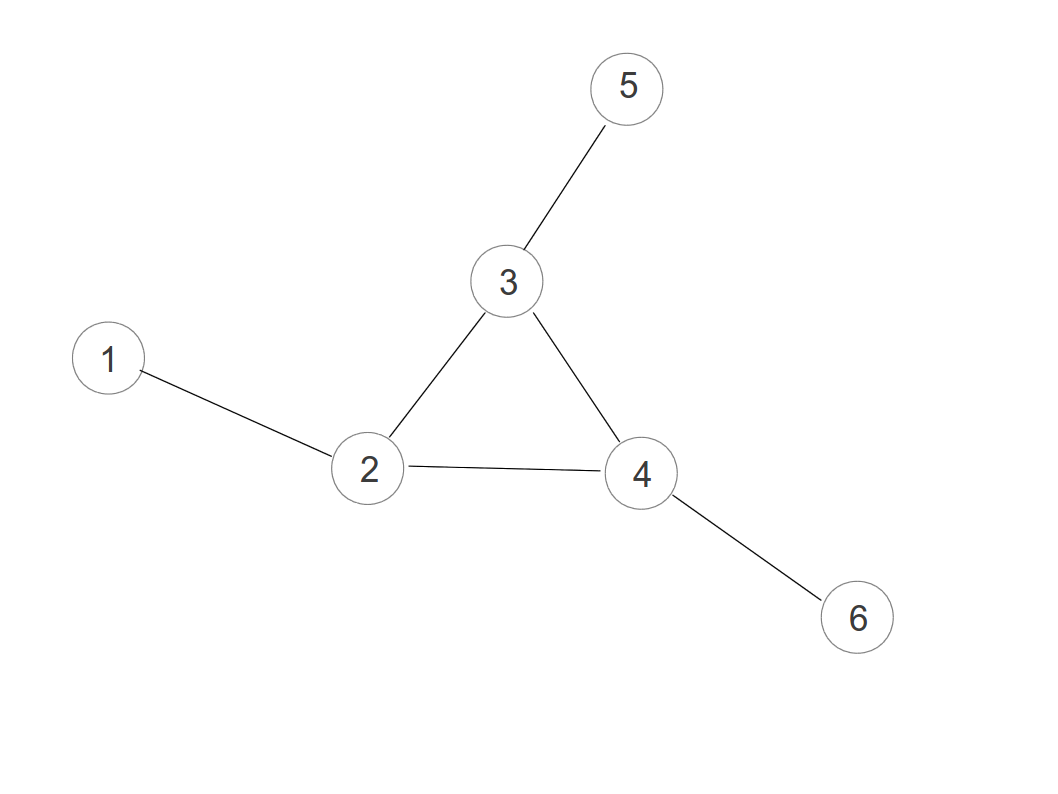
\includegraphics[scale=0.3]{exacto/imgs/ejemplito.png}}
  \subfloat[Frontera=4.]{
   \label{}
    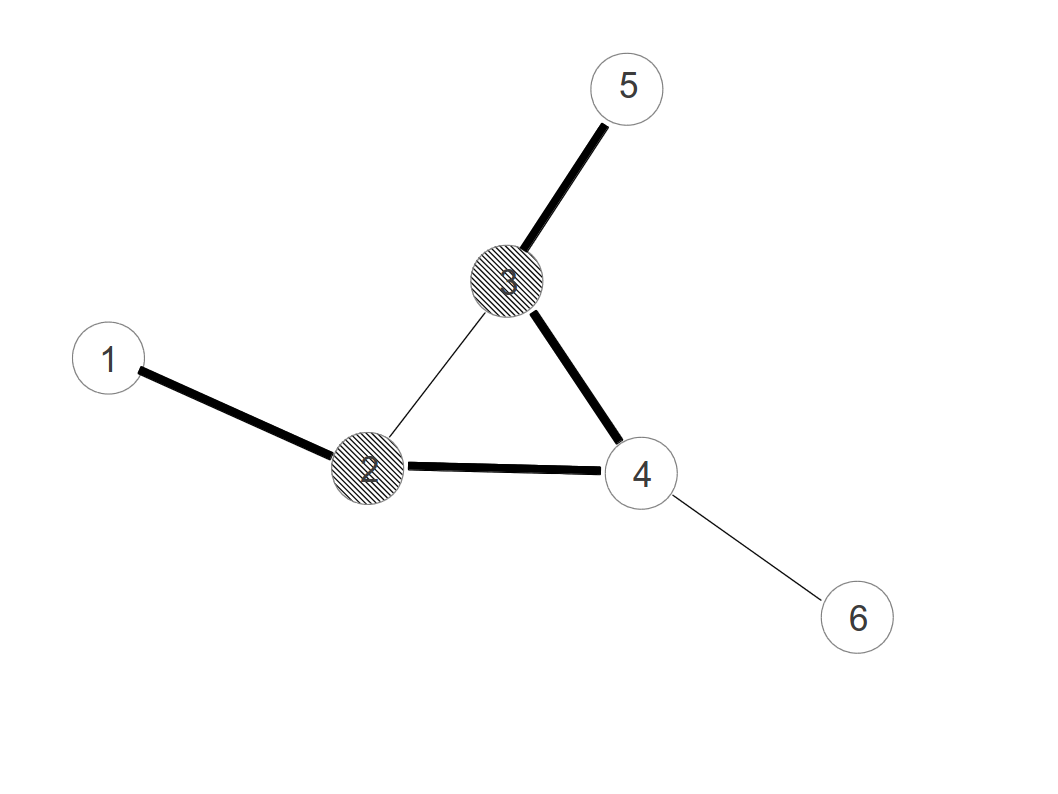
\includegraphics[scale=0.3]{exacto/imgs/ejemplitoSol.png}}
\caption{Un ejemplo y su solución}

\end{figure}

\begin{center}
    \begin{tabular}{ | l | l | l | l | l | p{5cm} |}
    \hline
    Llamada recursiva & R & P & X & cliqueMaxFrontera & Comentarios \\ \hline
    1 & $\{$ $\}$ & $\{$1,2,3,4,5,6$\}$ & $\{$ $\}$ & $\{$ $\}$ & Candidatos: todos los nodos del grafo. \\ \hline
    2 & $\{$1$\}$ & $\{$2$\}$ & $\{$ $\}$ & $\{$1$\}$ Frontera: 1 & Formo la clique R y el único candidato posible es el nodo 2 (único adyacente).\\ \hline
    3 & $\{$1,2$\}$ & $\{$ $\}$ & $\{$ $\}$ & $\{$1,2$\}$ Frontera: 2 & La clique R no puede agregar más nodos. Los adyacentes a 2 no son adyacentes a 1. \\ \hline
    4 & $\{$2$\}$ & $\{$3,4$\}$ & $\{$1$\}$ & $\{$2$\}$ Frontera: 3 & La clique R tiene dos candidatos para agregar (sus adyacentes) pero no puede agregar el nodo 1 que se encuentra en X ya que esa clique ya fue analizada previamente.\\ \hline
    5 & $\{$2,3$\}$ & $\{$4$\}$ & $\{$ $\}$ & $\{$2,3$\}$ Frontera: 4 & Candidato: 4. Adyacente a 2 y 3.\\ \hline
    6 & $\{$2,3,4$\}$ & $\{$ $\}$ & $\{$ $\}$ & $\{$2,3$\}$ Frontera: 4  &\\ \hline
    7 & $\{$2,4$\}$ & $\{$ $\}$ & $\{$ $\}$ & $\{$2,3$\}$ Frontera: 4 & El 3 no es candidato ya que fue evaluada esa opción previamente. \\ \hline
    8 & $\{$3$\}$ & $\{$4,5$\}$ & $\{$ $\}$ & $\{$2,3$\}$ Frontera: 4 & El 2 no es candidato ya que fue evaluada esa opción previamente.\\ \hline
    9 & $\{$3,4$\}$ & $\{$ $\}$ & $\{$ $\}$ & $\{$2,3$\}$ Frontera: 4 & \\ \hline
    10 & $\{$3,5$\}$ & $\{$ $\}$ & $\{$ $\}$ & $\{$2,3$\}$ Frontera: 4 & \\ \hline
    11 & $\{$4$\}$ & $\{$6$\}$ & $\{$ $\}$ & $\{$2,3$\}$ Frontera: 4 & \\ \hline
    12 & $\{$4,6$\}$ & $\{$ $\}$ & $\{$ $\}$ & $\{$2,3$\}$ Frontera: 4 & \\ \hline
    13 & $\{$5$\}$ & $\{$ $\}$ & $\{$ $\}$ & $\{$2,3$\}$ Frontera: 4 & \\ \hline
    14 & $\{$6 $\}$ & $\{$ $\}$ & $\{$ $\}$ & $\{$2,3$\}$ Frontera: 4 & \\
	\hline
    \end{tabular}
\captionof{table}{Seguimiento del algoritmo. Solución devuelta: $\{$2,3$\}$, frontera: 4.}
\end{center}



\newpage

\section{Algoritmo Goloso}
\subsection{Explicación del algoritmo implementado}
La heurística golosa que implementamos consiste en buscar el nodo de mayor grado del grafo. A partir de ese nodo v, se construye una clique de frontera máxima de la siguiente manera:

\begin{algorithm}[H]
\caption{Goloso}\label{ej2}
\begin{algorithmic}[1]
\Procedure{Goloso}{$G=(V,E)$}
	\State clique  $\shortleftarrow$ $\{$v nodo de mayor grado$\}$
	\While{ $\{Aumente frontera\}$ }
		\State $\{$Buscar nodo u$\}$ tal que u $\in$ nodos de la frontera y $ d(u) \ge d(p)$ $ \forall p \neq u $ y forme clique con nodos de clique
		\State clique $\cup$ $\{u\}$
	\EndWhile
	\State return |frontera|, |clique|, clique 
\EndProcedure
\end{algorithmic}
\end{algorithm}
Veamos con más detalle ciertos procedimientos para facilitar luego el análisis de complejidad.

Linea 4: Conseguir nodo candidato es básicamente intersecar los adyacentes de cada nodo de la clique que se tiene hasta el momento y luego tomar aquel de mayor grado. ¿Por qué la intersección de los adyacentes?. Porque me aseguro de obtener los nodos de la frontera que sean adyacentes a los nodos de la clique, lo que me permite agrandarla.
¿Por qué el de mayor grado?. Porque será el que mas nodos aporte a la nueva clique del resto de los nodos obtenidos en la intersección.
La intersección entre dos grupos de elementos consiste en recorrer uno de estos grupos y devolver aquellos que tienen coincidencias contra todos los elementos del otro grupo.

Linea 7: Calcular el tamaño de la \textit{frontera} consiste en sumar la cantidad de adyacentes de cada nodo de la clique y restar a este último número resultate las aristas de la clique (que son$ \displaystyle\frac{n(n-1)}{2}$).  

%%%%%%%%%%%%%%%%%%%%%%%%%%%%%%%%%%%%%%%%%%%%%%%%%%%%%%%%%%%%%%%%%%%%%%%%%%%%%%%%%%%%%%%%%%%%%%%%%%%%%%%%%%%%%%%%%%%%%%%%%%%%%%%%%%%%%%%%%%%%%%
%%%%%%%%%%%%%%%%%%%%%%%%%%%%%%%%%%%%%%%%%%%%%%%%%%%%%%%%%%%%%%%%%%%%%%%%%%%%%%%%%%%%%%%%%%%%%%%%%%%%%%%%%%%%%%%%%%%%%%%%%%%%%%%%%%%%%%%%%%%%%%

\subsection{Complejidad}
Veremos la complejidad de la heurística golosa siguiendo paso a paso el algoritmo:
\begin{itemize}
 \item En la linea 2, conseguir el nodo de mayor grado es O(n) pues se recorren todos los nodos.
 \item En la linea 3, se hacen a lo sumo n iteraciones (puede que la clique de frontera máxima sea el grafo entero), luego O(n).
 \item En la linea 4, buscar el nodo candidato tiene una complejidad O($n^{3}$).
\end{itemize}

Luego podemos concluir que la complejidad de la heurística es polinómica (más precisamente O($n^{4}$)). 

\begin{center}
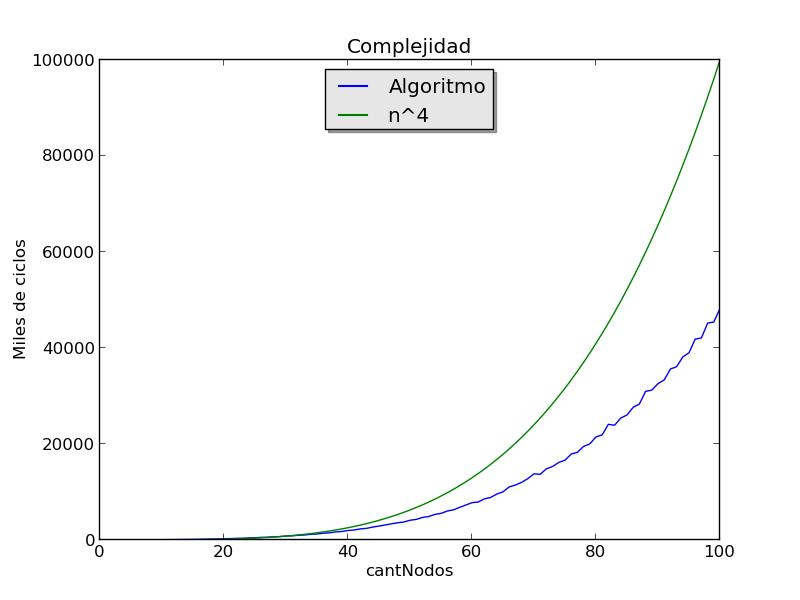
\includegraphics[scale=0.5]{goloso/grafico.jpg} 
\end{center}
El gráfico de complejidad fue realizado en base a grafos completos para asegurarnos que el algorítmo no supere la cota de complejidad en casos con muchas aistas y muchos nodos.
%%%%%%%%%%%%%%%%%%%%%%%%%%%%%%%%%%%%%%%%%%%%%%%%%%%%%%%%%%%%%%%%%%%%%%%%%%%%%%%%%%%%%%%%%%%%%%%%%%%%%%%%%%%%%%%%%%%%%%%%%%%%%%%%%%%%%%%%%%%%%%
%%%%%%%%%%%%%%%%%%%%%%%%%%%%%%%%%%%%%%%%%%%%%%%%%%%%%%%%%%%%%%%%%%%%%%%%%%%%%%%%%%%%%%%%%%%%%%%%%%%%%%%%%%%%%%%%%%%%%%%%%%%%%%%%%%%%%%%%%%%%%%

\subsection{Casos nefastos}

Los casos en que esta heurística falla, son aquellos en que el nodo de mayor grado del grafo no se encuentra dentro de la clique que se busca. 
¿Cuán mala puede ser? Tan mala como uno quiera, basta formar, por ejemplo, una estrella con el nodo central de grado máximo y una clique de fontera máxima con tamaño menor al grado máximo. Como ejemplo ilustrativo, mirar la siguiente imagen.
\begin{center}
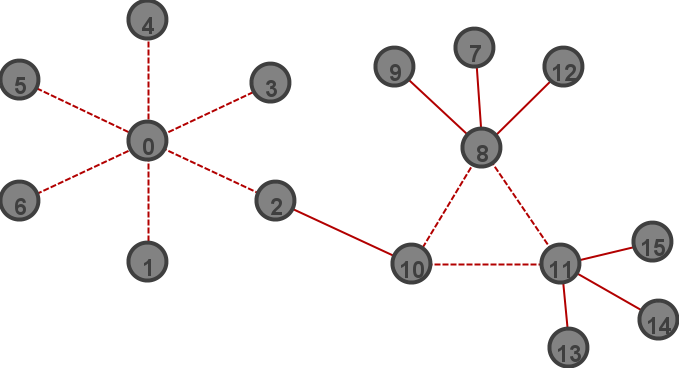
\includegraphics[scale=0.5]{goloso/labl.png} 
\end{center}


\newpage

\section{Algoritmo Busqueda Local}
\subsection{Explicaci\'on del algoritmo}

Para desarrollar el algoritmo de Búsqueda local, necesitamos definir dos cosas. Una es la \"vecindad\" y la otra cual será nuestra solución inicial.

Consideramos que una clique es vecina de otra si difieren exactamente en un nodo, es decir puede tener un nodo más, un nodo menos o uno distinto (con el mismo número de nodos). Si la clique posee un único nodo, sólo se tienen en cuenta los vecinos que tienen un nodo más, porque no podemos sacar (nos quedaríamos sin solución), y para cambiar un nodo lo que hacemos es primero quitar uno, y después poner uno entre todas las posibilidades que en este caso serían todos los nodos, por lo tanto elegiría el nodo de mayor grado, y justamente no buscamos que empiece por ahí.

La solución inicial es un nodo elegido al azar.
En cada iteración creamos la vecindad de la clique de máxima frontera (CMF) hasta el momento, recorremos sus vecinos y en caso de que tenga mayor frontera que la CMF hasta el momento, ésta pasa a ser la nueva CMF.

Otras vecindades que tuvimos en cuenta fueron:
\begin{itemize}
\item Cliques de igual o diferencia de uno en tamaño.
\item La clique de mayor tamaño que contenga a todos los nodos que forman parte de la solución en ese momento. La consideramos junto con la definición de vecindad que terminamos implementando.
\end{itemize}

Las descartamos porque los algoritmos para encontrar estas cliques vecinas implican una complejidad muy alta, y el proceso para hacerlo no resulta tan directo como el que elegimos, que si bien puede llegar a evaluar un gran número de posibilidades, está muy relacionado con el grado de los nodos y cantidad que tengamos en la solución, ya que si agregamos un nodo será uno de la frontera, si sacamos será uno de la solución que teníamos y si intercambia será entre uno de la solución con uno de la frontera.

La solución inicial es elegida al azar porque nos dimos cuenta que si empezábamos por el nodo de mayor grado, el resultado que obteníamos era el mismo que con la heurística constructiva del algoritmo goloso, al menos para la gran mayoría de familias de grafos.

\textbf{Ejemplo del funcionamiento:}

\begin{center}
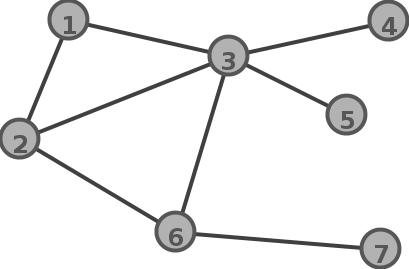
\includegraphics[scale=0.5]{Images/ejemploGrafo.png} 
\end{center}

Dado el siguiente grafo y comenzando por el nodo 4 (elegido al azar) el algoritmo realiza las siguientes iteraciones:
\begin{center}
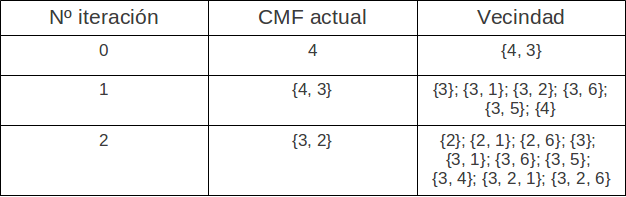
\includegraphics[scale=0.7]{Images/EjemploLocal.png} 
\end{center}

Y el resultado final, que también es el esperado, es: $\lbrace $3, 2$\rbrace$ que tiene una frontera de 6.

\subsection{Pseudoc\'odigo y complejidad}
\begin{algorithm}
	\caption{Busqueda Local}\label{local}
	\begin{algorithmic}[1]
	\Procedure{Local }{$G\ =\ (V,\ E)$}
		\State $CMF=\ random(nodos)$	\Comment{elige un nodo al azar}
		\While{$hay\_ cambio$}			\Comment{si no hay cambios CMF es máx local}
			\State $armar\_ vecindad(CMF)$
			\ForAll{$vecino\ in\ vecindad$}
				\If{$frontera(vecino)\ >\ frontera(CMF)$}
					\State $CMF=\ vecino$
				\EndIf
			\EndFor
		\EndWhile
	\EndProcedure
	\State

	\Procedure{armar\_vecindad}{$Clique\ =\ (V,\ E)$}
		\If{$|V|\ >\ 1$}
			\ForAll{$nodo\ in\ V$}
				\State $vecindad\_agregar(Clique-nodo)$
\Comment{Cliques vecinas con un nodo menos}
				\ForAll{$nodo\_candidato\ in\ nodos\_candidatos(Clique-nodo)$}
					\State $vecindad\_agregar(Clique-nodo+nodo\_candidato)$
\Comment{Cliques vecinas con un nodo intercambiado}
				\EndFor
			\EndFor
		\EndIf
		\ForAll{$nodo\_candidato\ in\ nodos\_candidatos(Clique)$}
			\State $vecindad\_agregar(Clique+nodo\_candidato)$
\Comment{Cliques vecinas con un nodo más}
		\EndFor
	\EndProcedure
\end{algorithmic}
\end{algorithm}

nodos\_candidatos(Clique): retorna un vector con los nodos de G que se pueden agregar a la Clique de forma que esta siga siendo un grafo completo.

\textbf{Complejidad: }

La función nodos\_candidatos debe recorrer los nodos de la clique y calcular la intersección entre todos los adyacentes de estos. Por lo tanto una cota holgada para esta función sería O($n^3$). 
Holgada porque si hay n nodos en la clique, no hay más nodos para agregar, por lo tanto la intersección entre los dos primeros sería vacío y no tiene porque continuar.

Luego, la función armar\_vecindad recorre los nodos de la clique (linea 15), llama a nodos\_candidatos dos veces (lineas 17 y 22) y los recorre una vez (linea 22). 
La cantidad de nodos de la clique es a lo sumo n y los nodos candidatos también. Entonces su complejidad es: O(n)*O(n\^{3}) + O(n) = O($n^4$).

Por último la función local, llama a armar\_vecindad (linea 4) y recorre la vecindad (linea 5) una vez por iteración, mientras haya cambio.

El tamaño de la vecindad está dado por la siguiente cuenta, en una clique de k nodos:

\begin{center}
\begin{tabular}{  c  c  }
(vecinos que tienen un nodo menos) & k elecciones
\\ + & + \\ 
(vecinos que tienen un nodo intercambiado) & k*(n-k) elecciones
\\ + & + \\ 
(vecinos que tienen un nodo más) & (n-k) elecciones
\\ = & = \\
(cantidad de vecinos) & k + k*(n-k) + (n-k)
\end{tabular}
\end{center}

Si buscamos un k de forma que se maximize esa cuenta nos daremos cuenta que k=$n/2$ es el que sirve. Dejando así como máximo tamaño de la vecindad $(n^2/4) +n$. Es decir, recorrer la vecindad es O($n^2$).

Falta ver cuántas veces itera, es decir, cuando deja de haber cambio. En el peor de los casos, la frontera de mi clique va aumentando de a uno, entonces como mucho puede iterar cantidad de aristas (m) de veces.

Cuenta final= cantidad de iteraciones * (armar\_vecindad + recorrerla) = O(m) * (O($n^4$) + O($n^2$)) = O(m*$n^4$)

\subsection{Casos nefastos}


\subsection{Experimentaci\'on}






\section{Algoritmo Búsqueda Tabú}
\subsection{Explicaci\'on del algoritmo}
La metaheurística de Búsqueda Tabú, se basa en una heurística de Búsqueda Local y permite escapar de los óptimos locales para intentar encontrar mejores soluciones. Incorpora estructuras de memoria para llevar un registro que permite elegir vecindades evitando aquellas que ya fueron visitadas (de esta manera no se forman ciclos). Esta estructura es llamada lista Tabú, debemos definir que información de las soluciones que visitamos va a almacenar y en qué medida.

En nuestro algoritmo para implementar la lista Tabú primero pensamos en guardar las soluciones que iban surgiendo, pero fue descartada porque el número de soluciones que visitamos puede ser muy grande, si pensamos en que las cliques son conjuntos de nodos, entonces se podrían formar muchas combinaciones que tendremos que evaluar al momento de obtener un candidato.
Finalmente nos decantamos por almacenar nodos visitados, que nos permite acotar la lista en el número de nodos del grafo. Un nodo ingresa a la lista Tabú si fue apartado de la solución en el movimiento de una solución a una vecina. 

Por medio de un esquema podemos mostrar el funcionamiento de la metaheurística:
\begin{center}
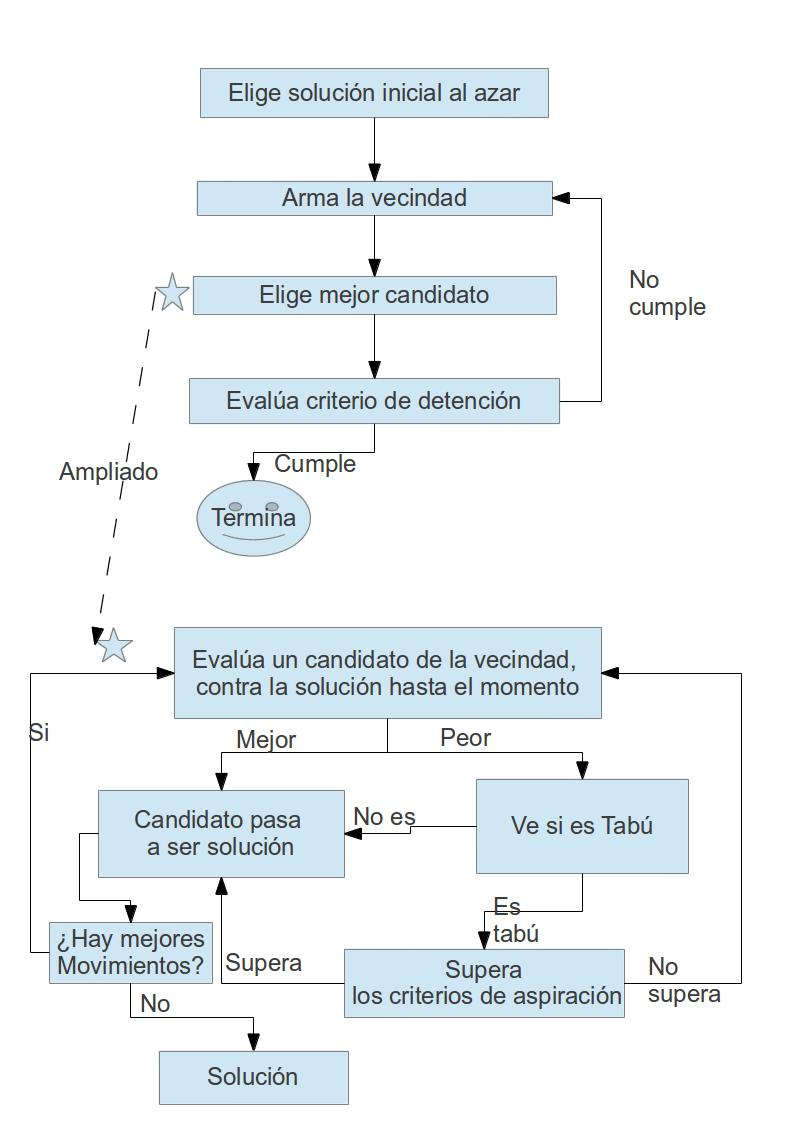
\includegraphics[scale=0.3]{tabu/esquema.jpg}
\end{center}

\subsection{Pseudoc\'odigo y complejidad}


\subsection{Casos nefastos}


%\subsection{Experimentaci\'on}







\end{document}
